
\documentclass[fleqn,12pt]{article}

\usepackage[margin=15mm]{geometry}
\usepackage[utf8]{inputenc}
\usepackage[bulgarian]{babel}
\usepackage[unicode]{hyperref}
\usepackage{amsfonts}
\usepackage{amssymb}
\usepackage{enumitem, hyperref}
\usepackage{upgreek}
\usepackage{indentfirst}
\usepackage{graphicx}

\usepackage{amsmath}

\graphicspath{ {./img/} }

\title{Тема 20 \\Проектиране и интегриране на софтуерни системи}

\author{v0.1}
\date{30 юни 2021}

\begin{document}

\maketitle
\tableofcontents
\pagebreak

\section{Характеристики на разпределените софтуерни системи}
\subsection{Дефиниции}

Налични са следните дефиниции:
\begin{itemize}
    \item Разпределена софтуерна система е като група от независими компютри, които за потребителя изглеждат като една цялостна система.
    \item Система, в която хардуерни или софтуерни компоненти, принадлежащи на компютри (възли), свързани в мрежа, комуникират един с друг и координират своите действия само чрез изпращане на съобщения.
\end{itemize}

\subsection{Видове системи}

Има следните видове:
\begin{itemize}
    \item разпределени изчислителни системи;
    \item разпределени информационни системи;
    \item широкоразпространени разпределени системи;
\end{itemize}

\textbf{\textit{Разпределените изчислителни системи}} се използват за изчислителни задачи изискващи висока производителност.
Има следните видове:
\begin{itemize}
    \item \textbf{Клъстер} - една програма работи паралелно върху много възли.
    Тези възли са идентични (откъм хардуер), с еднаква ОС, близко са разположени географски и са свързани в една мрежа.
    \item \textbf{Грид} - хетерогенни системи, където може ОС, хардуера или мрежата на възлите да се различават.
    Често възлите са отдалечени географски.
\end{itemize}

\textbf{\textit{Разпределените информационни системи}} се използват за свързване с множество приложения, които си комуникират по мрежата и може да са оперативно несъвместими.
Интеграцията на такива приложения е на няколко нива, като основните са:
\begin{itemize}
    \item \textbf{Client-Server} - на ниско ниво се позволява клиентите да групират заявки към сървър, които се изпълняват ''атомарно''.
    \item \textbf{Peer-to-Peer} - на по-високо ниво се позволява приложенията да комуникират едно с друго.
\end{itemize}

\textbf{\textit{Широкоразпространените разпределени системи (Pervasive distributed systems)}} за разлика от другите два вида, които са стабилни, са нестабилни.
Това се налага поради появата на мобилни и вградени изчислителни системи, където нестабилността е неимоверна.
Възлите в такива мрежи са мобилни, малки, черпещи енергия от батерии и обичайно ползват безжична връзка.
Характеризират се с липса на нужда от непрекъснат човешки надзор.

\subsection{Тенденции}

\begin{itemize}
    \item Използването на широкоразпространени мрежови технологии.
    \item Подобрява се интеграцията на малки и мобилни изчислителни устройства в разпределените системи. Такива са телефони, smartwatch, GPS устройства, табла на коли и други.
    \item Интернет е една голяма разпределена система, която постоянно се разширява.
    \item Увеличава се търсенето на мултимедийни услуги.
    \item Разпространение на on-demand разпределени системи.
\end{itemize}


\section{Междупроцесна комуникация}

Комуникацията между процеси се извършва чрез обмен на съобщения (Inter Process Communication (IPC)). ОС предоставя възможност за имплементация на IPC чрез механизми като:
\begin{itemize}
    \item message queue
    \item семафори
    \item shared memory
\end{itemize}

IPC механизмите на ОС обичайно не се използват директно, а посредством middleware програми, които служат като обвивка около тях, предоставящи абстракция чрез интерфейс.
Има два вида комуникация между процеси:
\begin{itemize}
    \item \textbf{connection-oriented} - чрез изграждане на канал специално за комуникацията;
    \item \textbf{message-oriented} - чрез преизползване на вече съществуващ канал за комуникация; 
\end{itemize}

Важна част от middleware представлява message-passing, който е механизъм за комуникация без използване на споделена памет.

\subsection{Отдалечено извикване}

Отдалечените извиквания представляват начин за използване на функционалност на процес A от процес B, като A извиква функционалност от B по прозрачен начин за себе си, т.е. замаскирвайки, че B е друг процес.
Може да се имплементира чрез \textbf{RPC} и \textbf{RMI}.
\bigbreak

\textbf{\textit{Remote procedure call (RPC)}} се базира на предоставянето на интерфейси, специфициращи процедури предлагани от друг процес.
По този начин се скрива реализацията на другия модул.
Интерфейсите се дефинират посредством \textbf{Interface Definition Language (IDL)}, който е проектиран с цел да позволи извикването процедура от един език в друг език.
\bigbreak
Семантиките на RPC са:
\begin{itemize}
    \item \textit{maybe} - отдалеченета процедура се изпълнява веднъж или въобще не се изпълнява.
    \item \textit{at-least-once} - клиентът получава резултат и знае, че процедурата се изпълнява поне веднъж, или получава информация за липса на резултат.
    \item \textit{at-most-once} - клиентът получава резултат и знае, че процедурата се е изпълнила най-много веднъж, или получава информация за липса на резултат.
\end{itemize}

\textbf{\textit{Remote method invocation (RMI)}} е обектно-ориентиран метод за отдалечено извикване методи.
\bigbreak
\textbf{RMI} прилича на \textbf{RPC} по това, че:
\begin{enumerate}
    \item Поддържа програмиране с интерфейси;
    \item Базира се на протокол заявка-отговор;
    \item Поддържа подобно ниво на прозрачност;
\end{enumerate}

\textbf{RMI} се различава от \textbf{RPC} по това, че:
\begin{enumerate}
    \item Позволява работа с обектно-ориентираната парадигма;
    \item Предоставя възможност за предаване референции към обекти като параметри;
\end{enumerate}

\begin{center}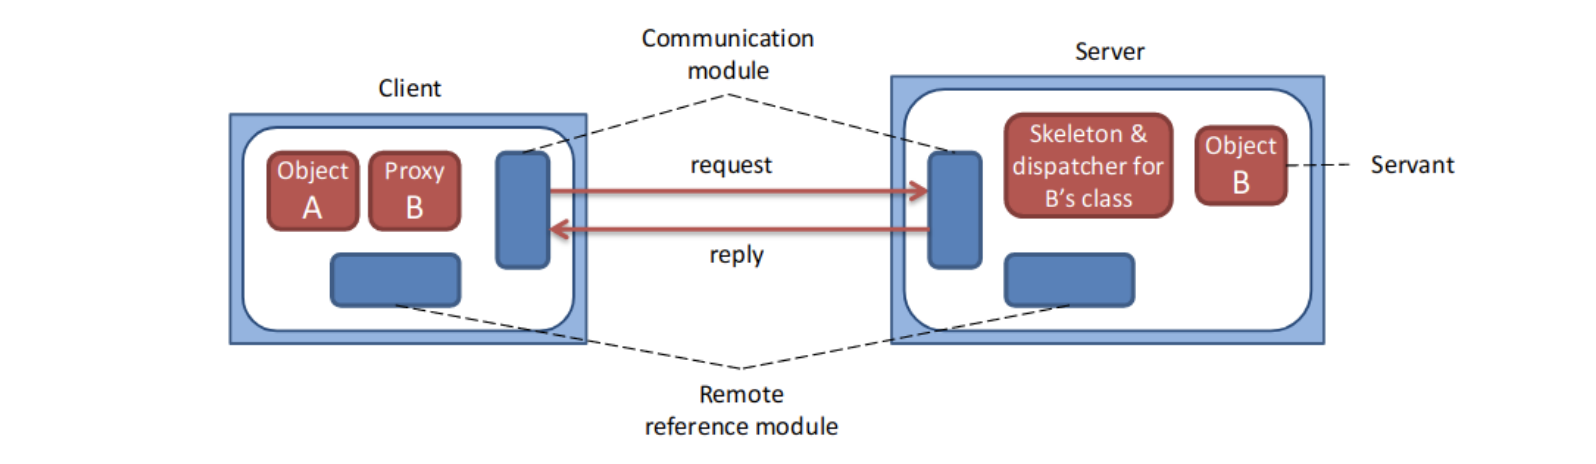
\includegraphics[width=350px]{rmi.png}\end{center}

Реализацията на \textbf{RMI} включва:
\begin{itemize}
    \item \textbf{Комуникационен модул}, който препраща заявките и отговорите между клиента и сървъра и осигурява семантиката на съобщението.
    От страна на сървъра комуникира с dispatcher-а на класа за извикания обект.
    \item \textbf{Remote reference module}, който e отговорен за съпоставката между локалните и отдалечените референции на обекти, създаването на отдалечени референции, както и тяхната маршализация/демаршализация.
    \item \textbf{Servant} - инстанция на отдалечен обект.
    \item \textbf{Proxy/Stub} - имплементира отдалечения интерфейс от страна на клиента, като служи за препращане на заявките за извикване на методи към съответния отдалечен обект. 
    \item \textbf{Skeleton} - имплементира отдалечения интерфейс от страна на сървъра, като делегира работата на \textbf{Servant}.
    \item \textbf{Dispatcher} - получава заявките от комуникационния модул и използва идентификатора на заявената операция за да извика съответния метод на \textbf{Skeleton} обекта.
\end{itemize}

\subsection{Мултикаст}

\textbf{\textit{Мултикаст}} представлява начин за изпращане на информация от един до много възли в една мрежа.
Топологията на тази мрежа може да бъде образувана като възлите оформят:
\begin{itemize}
    \item \textbf{дърво} и има директен достъп между всеки два възела;
    \item \textbf{mesh} и може да има няколко пътя от един връх до друг;
\end{itemize}

При мултикаст рутерите не се броят за възли, следователно може рутирането да не е толкова оптимално както на мрежовото ниво.
\bigbreak

Разпространението на информацията се оптимизира посредством алчния алгоритъм/техника \textbf{gossip (Gossip-Based Data Dissemination)}, където аналогично на разпространението на ковид/ебола всеки възел предава информацията на съседите си.
Възел, който държи информация се нарича \textit{заразен}, като той може да я предаде на своите съседи.
При епидемологичните алгоритми предаването на информация за това кога да се изтрие информация е трудно.
Следователно се симулира изтриването на информация чрез нейното модифициране.

\section{Разпределени неща}
\subsection{Разпределени обекти}
\subsection{Разпределени компоненти}

\section{Уеб услуги}
\subsection{Дефиниции}
\subsection{Шаблони за комуникация}
\subsection{Стандарти за уеб услуги}
\subsubsection{SOAP}
\subsubsection{WSDL}
\subsubsection{UDDI}

\end{document}
